
\subsection{Methodology}

All of our implementations were written in Java. Initially we thought of measuring the performance of our implementations with a naive approach where we would measure the time either in milliseconds or nanoseconds for sorting the input array. We could for example simply use \texttt{System.currentTimeMillis()} or \texttt{System.nanoTime()}. However we quickly found out how unreliable the results would be, since we noticed really inconsistent results between runs. As Ponge\cite{architectBenchmarking} explains, this kind of benchmarking might be viable in programs written in statically compiled languages like C. However Java runs on a Virtual Machine and it uses \emph{Just-in-time} compilation, so the first time the code is run it is actually being interpreted and then is compiled to native code, depending on the actual platform that is running. Furthermore, the VM tries to use all kinds of different optimization like loop unrolling, inlining functions or on-stack replacements, making it difficult to get consistent results. \\
We decided to use Java Microbenchmark Harness (JMH)\footnote{http://openjdk.java.net/projects/code-tools/jmh/} for measuring the performance of our implementations. JMH is an open source benchmarking tool part of the OpenJDK. Although it does not entirely prevent all common pitfalls and inconsistencies introduced by the JVM, it does help mitigating them. \\
Next step was to use the generated test cases files as inputs for our benchmarks. There are different modes to run benchmarks in JMH. We decided to measure the average time of an operation in microseconds, where an operation is sorting the array for any given algorithm and input array. In this mode, JMH considers an iteration to be a slice of time running as many operations as possible, it measures the time for each operation and averages it. In order to avoid some of the JIT inconsistencies and other JVM  optimizations, JMH runs a few warm-up iterations. After that it runs, by default, 5 iterations where the results are actually recorded. For our measuring purposes we decided to run 3  five seconds warm-up iterations and 5 ten seconds actual iterations.\\

The overall benchmark running time was over 36 hours. This was because we had large data sizes and due to the bad performance of some sorting algorithms in their worst case such as Bubble sort. We had to exclude Insertion and Bubble sort when running the test cases with a data size of 10,000,000.

\subsection{Results}

We ran the benchmark suite on a machine with an 4-cores and 8 logical processors @ 3.4Ghz and 24Gb of DDR4 RAM @ 3,401Mhz. The benchmark result reports can be found at our GitHub project link\cite{GitHubProjectURL}. All the algorithms were run serially and nothing was parallelized. The benchmarks suite took around 36 hours where the majority of time was spent on Bubble and Insertion sorts since they were very slow. We ran data size of 10,000,000 for all the algorithms excluding Bubble and Insertions Sort; however, we did not include it since the results were linear with the data size and it was not adding any new information. We do have all the produces results and reports at our public GitHub repository \cite{GitHubProjectURL}. In the graphs that we will use in this section the title of the graph will be the test case, they X-Axis is the data size and the Y-Axis is the time it took to sort the test case in microseconds.

\subsubsection{Interesting Observations}

In this section we will highlight some of the interesting observations that we found from our benchmark results since we cannot include all our graphs in the report due to space limitations; however, you can refer to the complete results and graphs at our public GitHub repository \cite{GitHubProjectURL}. In \textit{Figure \ref{fig:allInDescendingOrder}} we can see how bubble sort and insertion sort are very inefficient when it comes to sorting data compared to other sorting algorithms as the size of data increases. This is both bubble sort and insertion sorts worst case. However, they also perform much worse than the other algorithms in their general case, so we had to remove them from some graphs in order to see how the other algorithms performed in comparison with each other.

\begin{figure}[!ht]
\centering
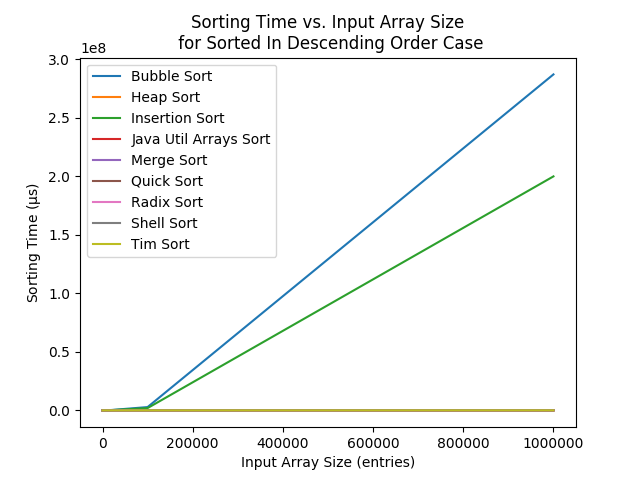
\includegraphics[width=9cm]{figures/plots_all_algs/sorting_time_vs_input_array_size_SortedInDescendingOrderCase.png}
\caption{Input case: data is sorted in descending order. All algorithms are included.}
\label{fig:allInDescendingOrder}
\end{figure}

Another interesting observation is shown in \textit{Figure \ref{fig:allButBubbleInAscendingOrder}} where the test case is of an array that is already sorted in ascending order which is bubble sort, insertion sort and shell sort best case. We can observe that insertion sort is as fast as the Java Utility Arrays Sort implementation, which is highly optimized, and see how, as expected, other sorting algorithms (like heapsort) still take a longer time to finish, even though the array is already sorted. Since shell sort's best case time complexity is $\Omega(n \lg n)$, it performs similarly to other algorithms like heapsort for which this is an average case input. Another interesting point, was that bubble sort did not perform as well as expected, and we had to take it out of the plot in order to see the details of the other algorithms. Bubble sort was expected to perform in $\Omega(n)$ in this case, but it was the algorithm that took the longest by far for all the input sizes. This was probably caused by a not very efficient implementation of the algorithm.

\begin{figure}[!ht]
\centering
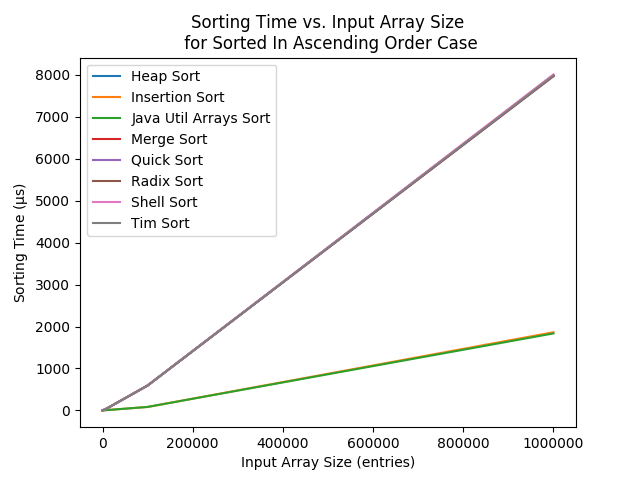
\includegraphics[width=9cm]{figures/plots_without_BubbleSort/sorting_time_vs_input_array_size_SortedInAscendingOrderCase.png}
\caption{Input case: data is sorted in ascending order. All algorithms included, except bubble sort.}
\label{fig:allButBubbleInAscendingOrder}
\end{figure}

In the case where the input consists of an array where all the values are the same (see \textit{Figure \ref{fig:allButBubbleSameValue}}), Java Util Arrays Sort and insertion sort performed the best. This was expected, since this is a sub-case of the best case scenario of insertion sort (the input is already sorted). Moreover, the optimization of the Java Util Arrays Sort is shown in the results of this input case, since the algorithm performs even better than insertion sort. However, bubble sort did not perform as well as expected for being its best case. It took so long, we had to remove it from the graph in order to see the details. of the other algorithms.

\begin{figure}[!ht]
\centering
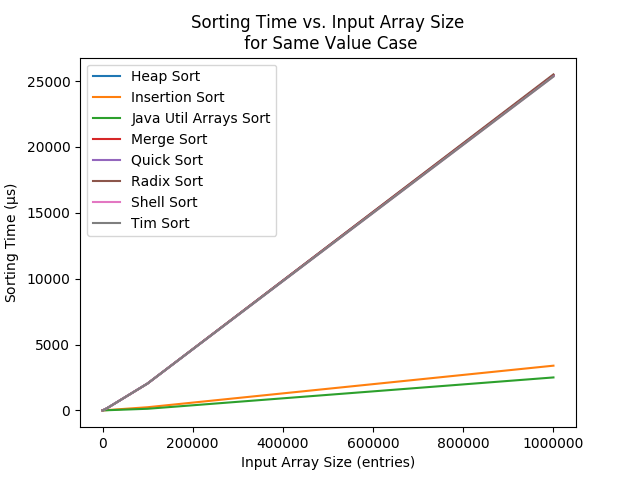
\includegraphics[width=9cm]{figures/plots_without_BubbleSort/sorting_time_vs_input_array_size_SameValueCase.png}
\caption{Input case: data is all the same value. All algorithms are included, except bubble sort.}
\label{fig:allButBubbleSameValue}
\end{figure}

In one of the input cases considered, we crafted the input array to be the worst case input for the mergesort algorithm. This input leads to the most comparisons possible when the mergesort algorithm is run. \textit{Figure \ref{fig:allButBubbleInsertionMergesortWorstCase}} shows this results, excluding bubble sort and insertion sort, so that mergesort's results are clearer. As expected, mergesort performed worst than the other algorithms for which this was an average case input. However, it did so by a small constant. This shows why mergesort is such a reliable algorithm. Mergesort has a consistent performance over all types of inputs, performing in $\Theta(n \lg n)$ even in the worst case.

\begin{figure}[!ht]
\centering
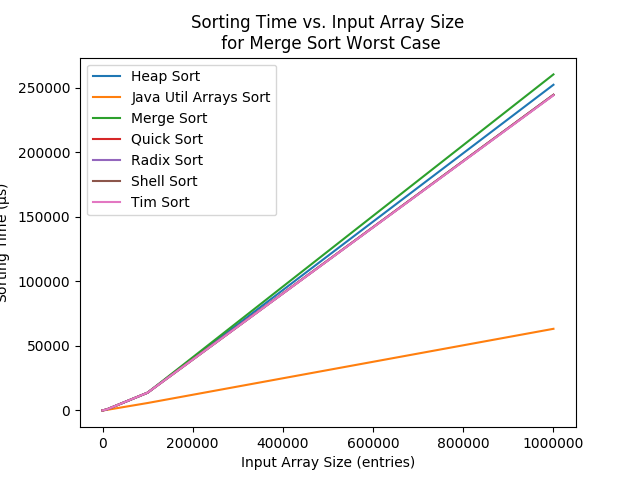
\includegraphics[width=9cm]{figures/plots_without_BubbleSort_InsertionSort/sorting_time_vs_input_array_size_MergeSortWorstCase.png}
\caption{Input case: data generated for mergesort's worst case input. All algorithms are included, except bubble sort and insertion sort.}
\label{fig:allButBubbleInsertionMergesortWorstCase}
\end{figure}

\subsubsection{Final Results Excluding Bubble and Insertion Sort}

Below are the results for all the test cases for all sorting algorithms except Bubble Sort and Insertion Sort since they are too slow compared to other sorting algorithms and would hide the relative differences between the other algorithms if included.

\begin{figure}[!htp]
\centering
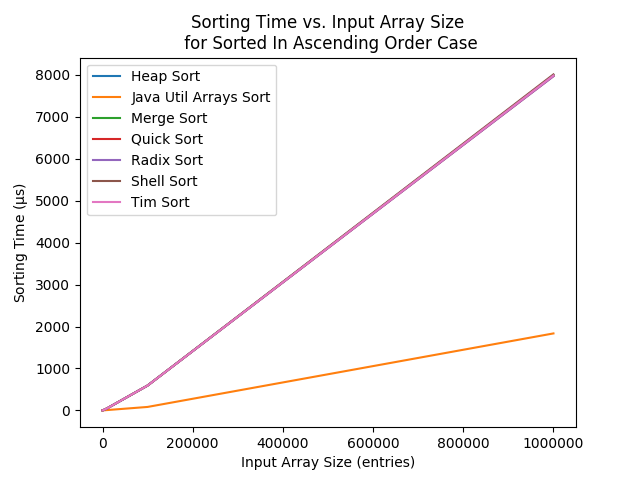
\includegraphics[width=9cm]{figures/plots_without_BubbleSort_InsertionSort/sorting_time_vs_input_array_size_SortedInAscendingOrderCase.png}
\end{figure}

\begin{figure}[!htp]
\centering
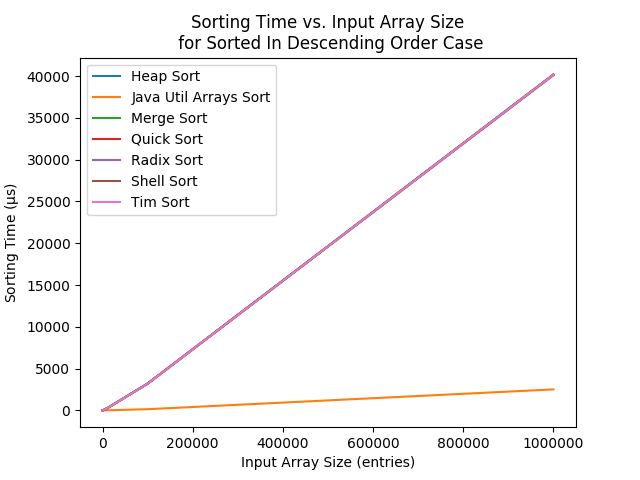
\includegraphics[width=9cm]{figures/plots_without_BubbleSort_InsertionSort/sorting_time_vs_input_array_size_SortedInDescendingOrderCase.png}
\end{figure}

\begin{figure}[!htp]
\centering
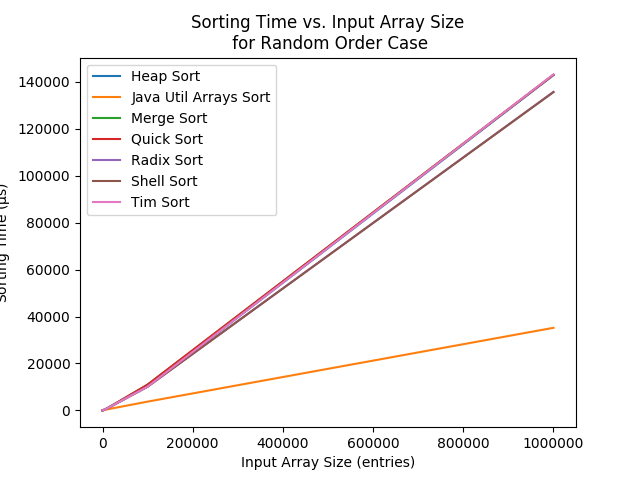
\includegraphics[width=9cm]{figures/plots_without_BubbleSort_InsertionSort/sorting_time_vs_input_array_size_RandomOrderCase.png}
\end{figure}

\begin{figure}[!htp]
\centering
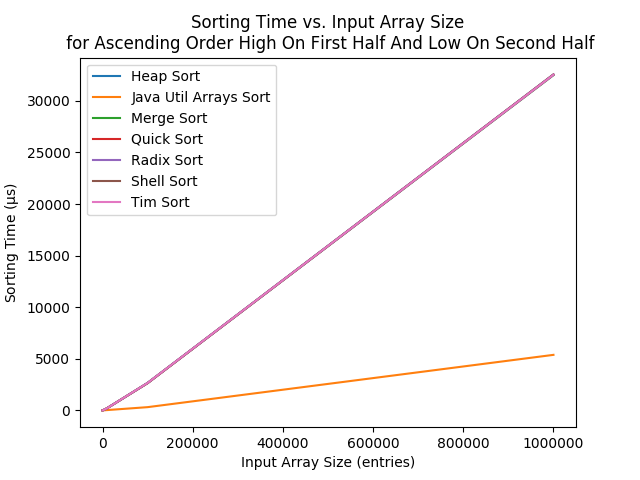
\includegraphics[width=9cm]{figures/plots_without_BubbleSort_InsertionSort/sorting_time_vs_input_array_size_AscendingOrderHighOnFirstHalfAndLowOnSecondHalf.png}
\end{figure}

\begin{figure}[!htp]
\centering
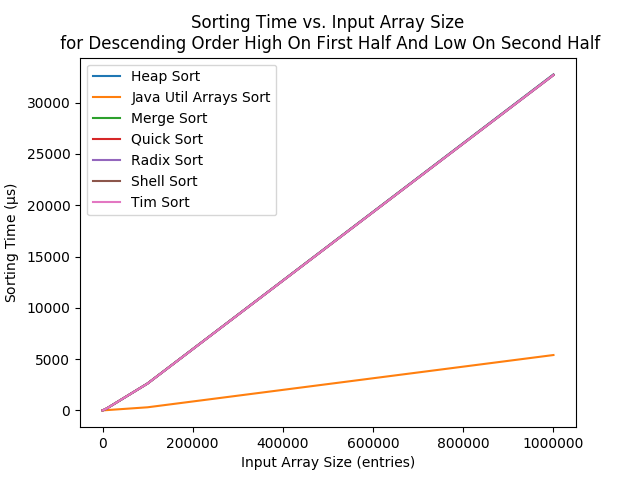
\includegraphics[width=9cm]{figures/plots_without_BubbleSort_InsertionSort/sorting_time_vs_input_array_size_DescendingOrderHighOnFirstHalfAndLowOnSecondHalf.png}
\end{figure}

\begin{figure}[!htp]
\centering
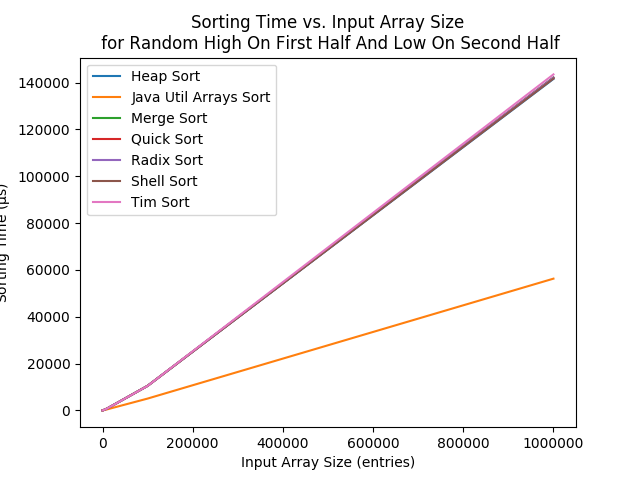
\includegraphics[width=9cm]{figures/plots_without_BubbleSort_InsertionSort/sorting_time_vs_input_array_size_RandomHighOnFirstHalfAndLowOnSecondHalf.png}
\end{figure}

\begin{figure}[!htp]
\centering
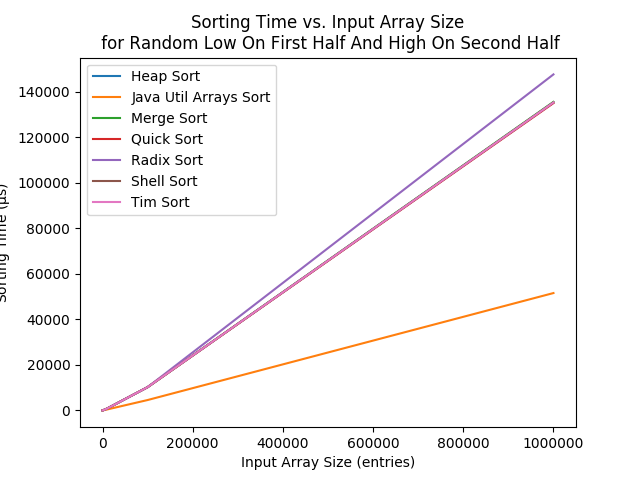
\includegraphics[width=9cm]{figures/plots_without_BubbleSort_InsertionSort/sorting_time_vs_input_array_size_RandomLowOnFirstHalfAndHighOnSecondHalf.png}
\end{figure}

\begin{figure}[!htp]
\centering
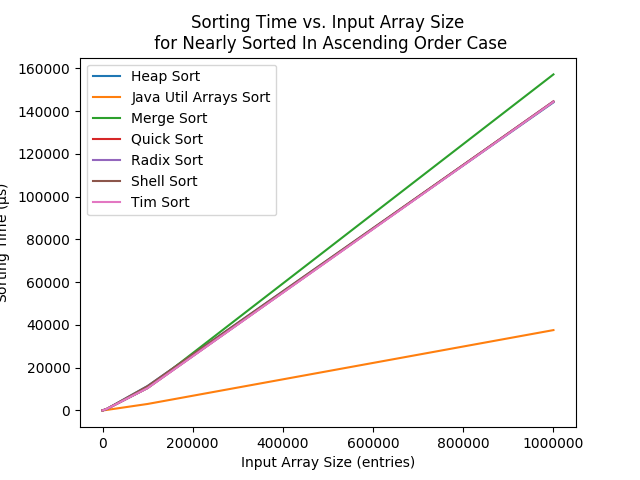
\includegraphics[width=9cm]{figures/plots_without_BubbleSort_InsertionSort/sorting_time_vs_input_array_size_NearlySortedInAscendingOrderCase.png}
\end{figure}

\begin{figure}[!htp]
\centering
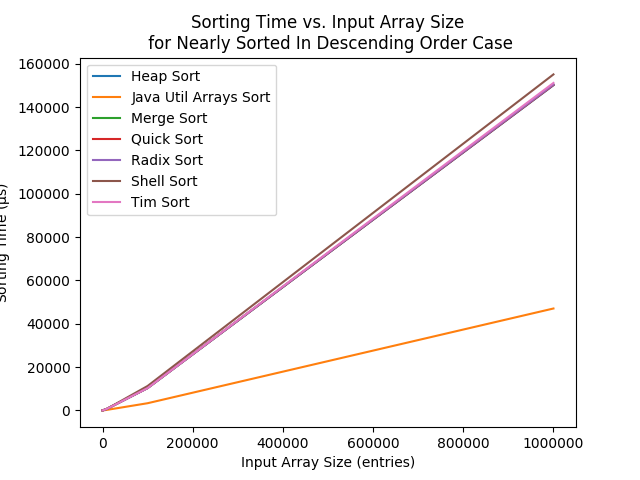
\includegraphics[width=9cm]{figures/plots_without_BubbleSort_InsertionSort/sorting_time_vs_input_array_size_NearlySortedInDescendingOrderCase.png}
\end{figure}

\begin{figure}[!htp]
\centering
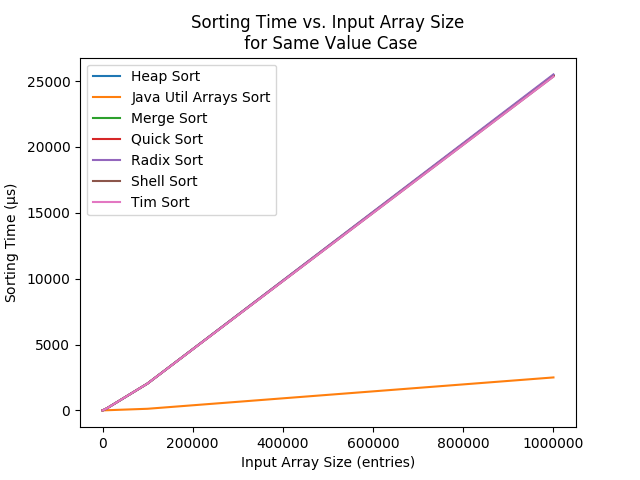
\includegraphics[width=9cm]{figures/plots_without_BubbleSort_InsertionSort/sorting_time_vs_input_array_size_SameValueCase.png}
\end{figure}
